\documentclass[a4paper, 12pt]{article}
\usepackage[top=2cm, bottom=2cm, left=2.5cm, right=2.5cm]{geometry}
\usepackage[utf8]{inputenc}
\usepackage{amsmath, amsfonts, amssymb, graphicx}
\begin{document}
\begin{center}
	\huge{Demonstração de Potêncial Elétrico}
\end{center}
\begin{center}
	Elias Sabát
\end{center}
\section{Definição de Potencial}
	Dado uma carga q fixa na origem, vamos calcular a integral da linha de campo elétrico sobre a curva que liga os pontos \textbf{a} e \textbf{b}.

\begin{center}
	\begin{figure}[!htb]
		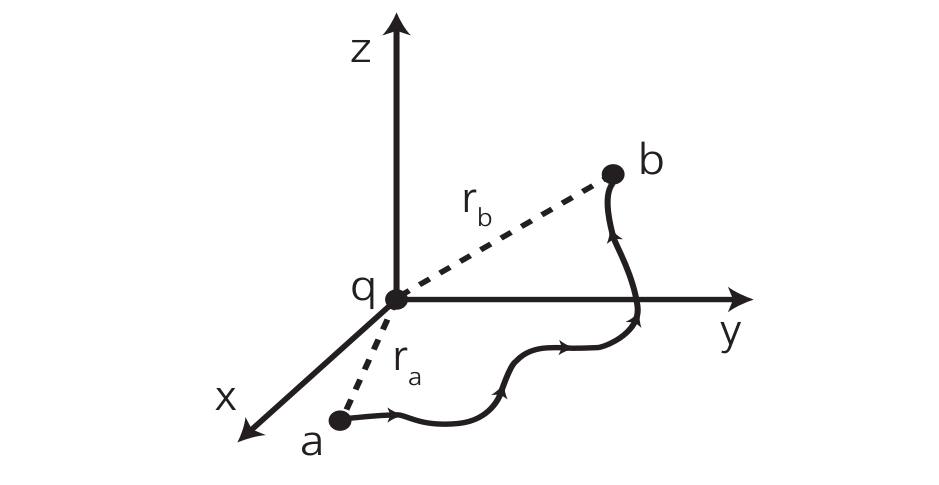
\includegraphics[scale=0.4]{figura1.png}
	\end{figure}
\end{center}

$$\int_{a}^{b}\vec{E} \cdot \vec{Dl}= \dfrac{q}{4\pi\epsilon_{0}}\int^{b}_{a}\dfrac{1}{r^2} \cdot \widehat{r} \cdot \vec{Dl} $$


tendo o seguinte detalhe em mente:
\begin{center}
	\begin{figure}[!htb]
		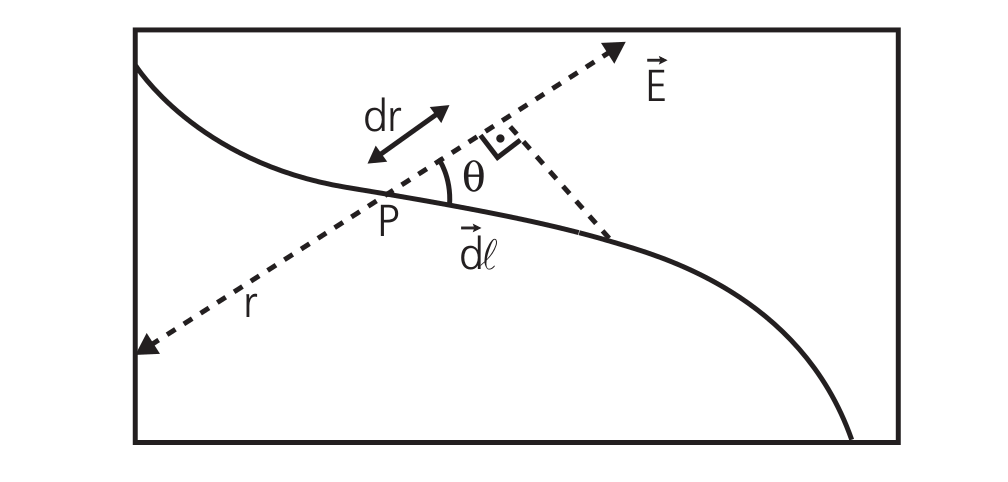
\includegraphics[scale=0.4]{figura2.png}
	\end{figure}
\end{center}
$$\widehat{r} \cdot \vec{Dl} = \vec{Dr}$$


sendo assim, temos: 

$$\int_{a}^{b}\vec{E} \cdot \vec{Dl} = \dfrac{q}{4\pi\epsilon_{0}}\int^{b}_{a}\dfrac{1}{r^2}\vec{Dr} = \dfrac{q}{4\pi\epsilon_{0}} \left(\dfrac{1}{r_{a} - r_{b}}\right)$$

\newpage

\section{Trabalho da Força Elétrica}

Vamos calcular o trabalho de \textbf{a} até \textbf{b} pela seguinte integral:

$$\varphi_{ab} = \int^b_{a} \vec{F}(r) \cdot \vec{Dr}$$

Para o caso da força elétrica sobre uma carga +q produzida
por uma carga pontual +Q localizada na origem, temos:

$$\varphi_{ab} = \dfrac{Qq}{4\pi\epsilon_{0}} \int^b_a\dfrac{1}{r^2}\vec{Dr} = \dfrac{Qq}{4\pi\epsilon_{0}} \left(\dfrac{1}{r_{a} - r_{b}}\right)$$

Da definição de Potencial Elétrico:

$$V(r) = \dfrac{Q}{4\pi\epsilon_{0}} \cdot \dfrac{1}{r}$$

Obtemos a energia potencial multiplicando o potencial
eletrostático pela carga de prova (carga que está sentindo o potencial):

$$U(r) = \dfrac{Qq}{4\pi\epsilon_{0}} \cdot \dfrac{1}{r}$$

A relação encontrada:

$$U(r) = qV(r)$$

Dessa forma, temos:

$$\varphi_{ab} = - [U(r_b) - U(r_a)] = - \Delta U$$

\begin{flushright}
Obrigado, Bons estudos!
\end{flushright}
	

\end{document}